\documentclass[titlepage]{article}
% preamble area, where packages used
\usepackage{amsmath} % package usage example

% paper setting
\setlength{\textwidth}{16.0cm}
\setlength{\textheight}{22.0cm}
\setlength{\oddsidemargin}{0.0cm}
\setlength{\topmargin}{0.0cm}

% ****paragraph and line setting****
% paragraph indentation
\setlength\parindent{0ex}
% paragraph skip: baselineskip=fontsize * baselinestretch, where fontsize is a constant corresponding to a chosen font type.
\setlength{\parskip}{0.5\baselineskip}
% line skip
\renewcommand{\baselinestretch}{1.5}

\usepackage{hyperref}
\usepackage[section,nottoc]{tocbibind}

\usepackage{graphicx}
\usepackage{rotating}
% declare the path(s) where your graphic files are
\graphicspath{{./fig/}}
% and their extensions so you won't have to specify these with
% every instance of \includegraphics
\DeclareGraphicsExtensions{.png}

\usepackage{amsmath}
\numberwithin{figure}{section}
\numberwithin{equation}{section}

\usepackage{algorithm}
\usepackage{algpseudocode}

\usepackage{comment}

\usepackage{xeCJK}
\setCJKmainfont{WenQuanYi Micro Hei Mono}

\begin{document}

\title{LTE PHY Benchmark Notes}
\author{Xuechao Wei}
\date{\today}
\maketitle

% main text

\section{LTE Background}

\textbf{Frame structure}\cite{erik}

The size of various fields in the time domain is expressed as a number of time units $T_{s}=1/(15000*2048)$.

Downlink and uplink transmissions are organized into radio frames with $T_{f}=3072000*T_{s}=10ms$ duration.

\textbf{Frame structure type 1}

$T_{f}=3072000*T_{s}=10ms$ long and consists of 20 slots of length $T_{slot}=15360*T_{s}=0.5ms$, numbered from 0 to 19. A subframe is defined as two consecutive slots where subframe $i$ consists of slots $2i$ and $2i+1$.

\textbf{TTI}

Data on a transport channel is organized into transport blocks. In each Transmission Time Interval (TTI), at most one transport block of a certain size is transmitted over the radio interface to/from a mobile terminal in absense of spatial multiplexing. In case of spatial multiplexing (MIMO), there can be up to two transport blocks per TTI.

Associated with each transport block is a Transport Format (TF), specifying how the transport block is to be transmitted over the radio interface. The transport format includes information about the transport-block size, the modulation scheme, and the antenna mapping. Together with the resource assignment, the resulting code rate can then be derived from the transport format. By varying the transport format, the MAC layer can thus realize different data rates. Rate control is therefore also known as transport-format selection.

LTE has inherited the basic principle of WCMA/HSPA that data are delivered to the physical layer in the form of Transport Blocks of a certain size. In terms of the more detailed transport-block structure, LTE has adopted a similar approach as was adopted for HSPA:

\subsection{LTE Downlink Scheme}

\textbf{Modulation}

如果想要传输一串输入数字信号(二进制bit流),就必须把这些信号放到正弦波上,因为无线信号在空气中是通过正弦波传输的,所以在把信号放到正弦波上以后,正弦函数的一些参量如振幅、频率、相位均可用来体现不同的信号值。

例如,如果正弦波的函数是

\begin{equation}
C*cos(f_{c}*t+\phi)
\end{equation}

以QAM为例,将上式展开一下化为

\begin{equation}
A*cos(f_{c}*t)+B*sin(f_{c}*t)
\end{equation}

现在希望将输入信号由A和B携带,这时就同时利用了振幅和相位来携带信息。如果A和B携带两个bit的信息,那么可以建立一个每两bit和一个实数的映射关系:

\begin{verbatim}
01-->1
10-->3
11-->-1
00-->-3
\end{verbatim}

如果将每两个实数分别作为一个复数的实部和虚部,那么一个复数就可以表示4bit的信息。进一步,如果将这个复数的实部和虚部分别对应于上面第2个式子中的A和B,那么就可以将每4bit的信息映射到一个正弦波上,这就完成了正弦波的信息携带。

我们需要做的只是一个映射工作,然后将每个复数的实部和虚部发送到发射电路,电路会完成“载波”的任务。相反,在接受端也会有一个滤波电路,将接受到的正弦波的A和B解出来然后发送给后面的解调及解码过程。

\textbf{OFDM}

OFDM的目的是将n个经过调制的频域信号转化为n个时域信号,每一个时域信号都由一系列间隔为$\Delta f$的子载波叠加而成,这些子载波相互正交。时域信号实际上是由n个频域信号时域化后采样得到。

假设经过基带调频并经过电路调制到高频之后,在$[0,T_{u}]$时间内,第$i$个子载波上已调的QAM信号可以表示为

\begin{equation}
	s_{i}(t)=A_{i_{c}}g(t)cos(2\pi f_{i}t)-A_{i_{s}}g(t)sin(2\pi f_{i}t)
=Re\{[A_{i_{c}}+jA_{i_{s}}]g(t)e^{j2 \pi f_{i}t}\}
=Re\{A_{i}g(t)e^{j2 \pi f_{i}t}\}
\end{equation}

其中,$A_{i}=A_{i_{c}}+jA_{i_{s}}$是发送的QAM符号的星座点,$A_{i_{c}}$和$A_{i_{s}}$分别是其同相分量(I路)和正交分量(Q路);$f_{i}=f_{c}+i\Delta f=f_{c}+{i\over T_{u}}$是第$i$路的载波频率,$i=0,1,...,N-1$;$g(t)$是脉冲成形滤波器的冲激响应,假设它为矩形脉冲。

总的OFDM信号可以表示为

\begin{equation}
	s(t)=\sum _{i=0} ^{N-1}s_{i}(t)
	=Re\{[\sum A_{i}g(t)e^{j{2 \pi}i{\Delta f}t}]e^{j{2 \pi}f_{c}t}\}
	=Re\{a(t)e^{j{2 \pi}f_{c}t}\}
\end{equation}

其中

\begin{equation}
	a(t)=\sum _{i=0}^{N-1}A_{i}g(t)e^{j{2\pi}i{\Delta f}t}
\end{equation}

是OFDM信号的复包络。

若令$I(t)=Re\{a(t)\}$,$Q(t)=Im\{a(t)\}$,则$s(t)$可以表示为

\begin{equation}
	s(t)=I(t)cos(2 \pi f_{c}t)-Q(t)sin(2 \pi f_{c}t)
\end{equation}

因此也可以先得到复包络$a(t)$,再经过I/Q\textbf{正交调制}来得到OFDM信号。

需要注意的是,对于BPSK、MASK这样的一维调制,所考虑的载波是$cos(2\pi f_{i}t)$,已调信号只有同相载波,没有正交载波$sin(2 \pi f_{i}t)$,因此载波正交的最小间隔是$1\over {2T_{u}}$,而不是$1\over {T_{u}}$。要保证同相载波和正交载波同时都正交,这就需要载波间隔为$1\over T_{u}$。由$s_{i}t$可见,对于二维调制,I路和Q路这两个载波可以表示为一个复数载波$e^{j2\pi f_{i}t}$(这里还不太理解)。对于两个复载波$c_{n}=g(t)e^{j2\pi f_{n}t}$和$c_{m}=g(t)e^{j2\pi f_{m}t}$,假设$g(t)$为矩形脉冲,则使$c_{n}(t)$和$c_{m}(t)$保持正交的最小间隔是$|f_{n}-f_{m}|=1\over T_{u}$。

为了实现OFDM调制的基带数字处理,首先要将OFDM信号的复包络进行采样,成为离散时间信号。

在$[0,T_{u}] (T_{u}={1\over {\Delta f}})$,$T_{u}=N*T_{samp}$,$T_{samp}$为采样频率的倒数。如果$N=2048$且$\Delta f = 15KHz$,则$T_{samp}=T_{s}$,$T_{s}$为time unit\cite{erik},大小为$1/(15000*2048)$。若采样时刻是$m{T_{u} \over N}, m=0,1,...,N-1$,则对OFDM信号的复包络$a(t)$采样后的序列为

\begin{equation}
	a_{m}=a(m{T_{u}\over N})=\sum _{i=0} ^{N-1} A_{i}e^{j2\pi i \Delta f m{T_{u} \over N}}
	=\sum _{i=0} ^{N-1}A_{i}e^{j2\pi {mi \over N}} \ m = 0,1,...,N-1
\end{equation}

该式恰好就是对序列$\{A_{0},A_{1},...,A_{N-1}\}$进行离散傅里叶反变换(IDFT)的结果。其中,IDFT得到的$N$个时间间隔为$T_{samp}$的一组输出叫做一个OFDM符号(OFDM symbol)。因此,给定输入的符号$\{A_{0},A_{1},...,A_{N-1}\}$后,借助IDFT即可得到OFDM复包络的时间采样。

接收端通过I/Q正交解调后可以恢复OFDM信号的复包络$a(t)$,将其采样得到的时间序列$\{a_{m}\}=\{a_{0},a_{1},...,a_{N-1}\}$。由于IDFT是可逆变换,因此对序列$\{a_{m}\}$进行离散傅里叶变换(DFT)即可得到发送的序列$\{A_{i}\}$:

\begin{equation}
	A_{i}=\sum _{m=0} ^{N-1}a_{m}e^{-j2\pi {mi\over N}} \ i = 0,1,...,N-1
\end{equation}

由于$\{a_{m}\}$是对时间信号的采样,故称其为时域序列。而$\{A_{i}\}$是序列$\{a_{m}\}$的离散傅里叶变换,故称其为频域序列。

当$N$为2的整幂时,DFT和IDFT存在快速算法:FFT和IFFT。这样,可以借助FFT和IFFT来实现OFDM信号的调制与解调。

\textbf{[Aside: ]}对\textbf{正交}、\textbf{频分}和\textbf{复用}的理解

我觉得\textbf{正交}包含两方面的含义,一指构成每个OFDM符号的各子载波彼此正交;二指往高频调制时,正交调制器附加的同相载波和正交载波相互正交。前者我需要关心,后者由调制电路来做,我不用管;\textbf{频分}是指各子载波的频率间隔为$\Delta f$;感觉\textbf{复用}最难理解,理想的正弦波的频谱其实是单值函数,即只在一个频率处有非零值,其它频率处都为0。但实际上由计算机生成的正弦波都是锯齿状的,看起来由许许多多的台阶构成,这就使得实际的“正弦波”频谱图如图2中的任意一个子载波所示,图中最高波峰即为我们所需要的理想正弦波频谱的那个非零值。传统的FDM做法是让每个子载波间隔足够大的$\Delta f$值,使得每个子载波的最大频谱波形彼此分开,如图1所示。而OFDM则保证只要用一个最小的$\Delta f$使子载波正交,就可以用如下函数将各子载波的最大非零频谱值区分出来(虽然彼此之间存在重叠干扰):

\begin{equation}
	s(f)=\left\{
		\begin{array}{ll}
			0 & \textrm{if $f=n\Delta f (n \neq 0)$} \\
			a_{0}+b_{0}j & \textrm{else}
		\end{array}
		\right.
\end{equation}

\begin{figure}[htbp]
	\centering
	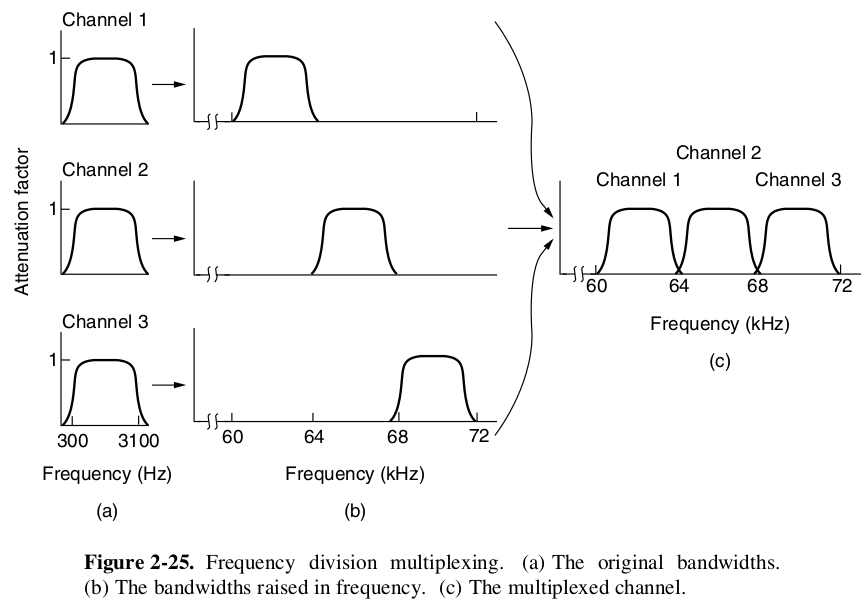
\includegraphics[height=3.14159in]{FDM}
	\caption{Traditional FDM}
\end{figure}

\begin{figure}[htbp]
	\centering
	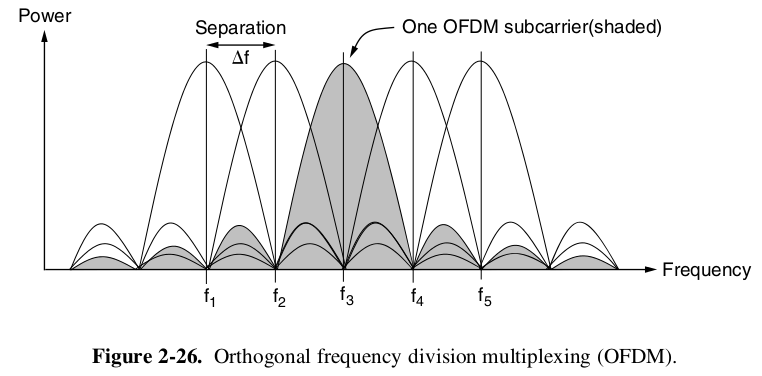
\includegraphics[height=2.5in]{OFDM}
	\caption{OFDM}
\end{figure}

当然,这只是非常粗略理解。

\textbf{CRC}

循环冗余校验是通过模2除法运算来建立有效信息位和校验位之间的约定关系。其中待编码的有效信息以多项式$M(x)$表示,将它左移若干位后,用另一个约定好的多项式$G(x)$去除,所产生的余数就是校验位。当接受方收到发来的CRC码后,他仍用约定的$G(x)$去除,若余数为0,表明该代码接受无误;若余数不为0,表明某一位出错,再进一步由余数值确定出错的位置,并予以纠正。

CRC的编码步骤如下:

\begin{itemize}
	\item 将待编码的$N$位有效信息位表示为一个$n-1$阶的多项式$M(x)$;
	\item 将$M(x)$左移$K$位,得到$M(x)x^{k}$($k$由预选的$k+1$位的生成多项式$G(x)$决定);
	\item 用一个预选好的$k+1$位的生成多项式$G(x)$对$G(x)x^{k}$做模2除法;
	\item 把左移$k$位后的有效信息位与余数做模2加法,即形成长度为$N+K$的CRC码。
\end{itemize}

\textbf{Turbo coding}

The transfer function of the 8-state constituent code for the PCCC (Parallel Concatenated Convolutional Code) is\cite{36series-212}:

\begin{displaymath}
	G(D)=[1,{g_{1}(D) \over g_{0}(D)}]
\end{displaymath}

where

\begin{displaymath}
	g_{0}(D)=1+D^{2}+D^{3} \\
	g_{1}(D)=1+D+D^{3}
\end{displaymath}

\begin{figure}[htbp]
	\centering
	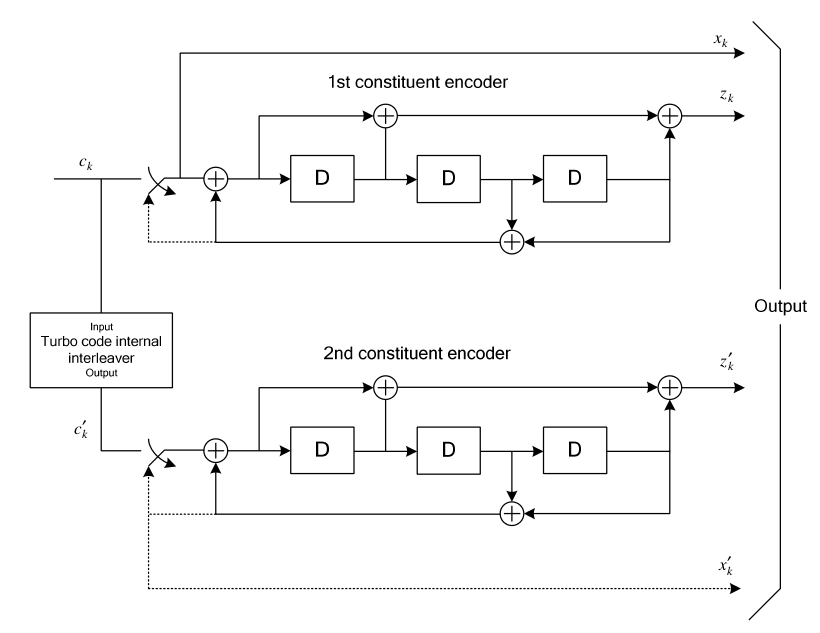
\includegraphics[height=3in]{turbo}
	\caption{Structure of rate 1/3 turbo encoder (dotted lines apply for trellis termination only)}
\end{figure}



\begin{itemize}
	\item In case of single-antenna transmission there is a single transport block of dynamic size for each TTI.

	\item In case of multi-antenna transmission, there can be up to two transport blocks of dynamic size for each TTI, where each transport block corresponds to one codeword in case of downlink spatial multiplexing. This implies that, although LTE supports downlink spatial multiplexing with up to four layers, the number of codewords and thus also the number of transport blocks is still limited to two.
\end{itemize}

\textbf{Channel mapping}

\begin{figure}[htbp]
	\centering
	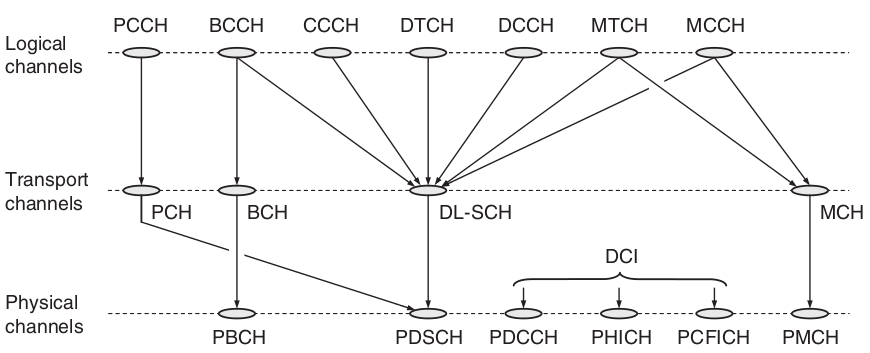
\includegraphics[height=2in]{DLCH}
	\caption{Downlink channel mapping}
\end{figure}

\begin{figure}[htbp]
	\centering
	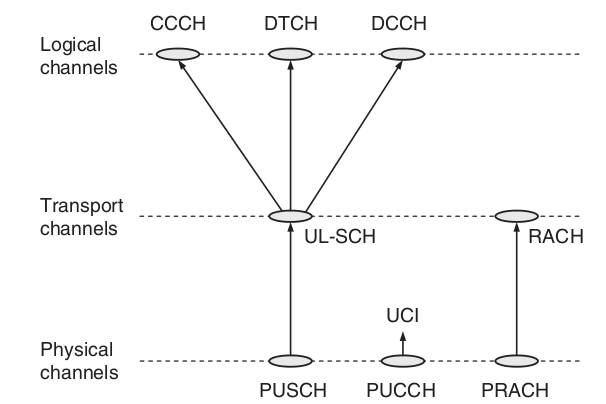
\includegraphics[height=2.2in]{ULCH}
	\caption{Uplink channel mapping}
\end{figure}

我对channel mapping的概念感到极其不理解,但从下面的文字中貌似可以看出transport channel和physical channel的联系:

To the transport block(s) to transmit on the DL-SCH, a CRC, used for error detection in the receiver, is attached, followed by Turbo coding for error correction. In case of spatial multiplexing, the processing is duplicated for each of the transport blocks. Rate matching is used not only to match the number of coded bits to the amount of resources allocated for the DL-SCH transmission, but also to generate the different redundancy versions as controlled by the hybrid-ARQ protocol.

After rate matching, the coded bits are modulated using QPSK, 16QAM, or 64QAM, followed by antenna mapping. The antenna mapping can be configured to provide different multi-antenna transmission schemes including transmit diversity, beam-forming, and spatial multiplexing. Finally, the output of the antenna processing is mapped to the physical resources used for the DL-SCH. The resources, as well as the transport-block size and the modulatin scheme, are under control of the scheduler.

A \textit{phsical channel} corresponds to the set of time-frequency resources used for transmission of a particular transport channel and each transport channel is mapped to a corresponding physical channel.

经过师兄的指点,现在的理解是,物理信道主要负责资源块的分配,传输信道负责前面的编码部分。

\textbf{The downlink physical resource}

\begin{figure}[htbp]
	\centering
	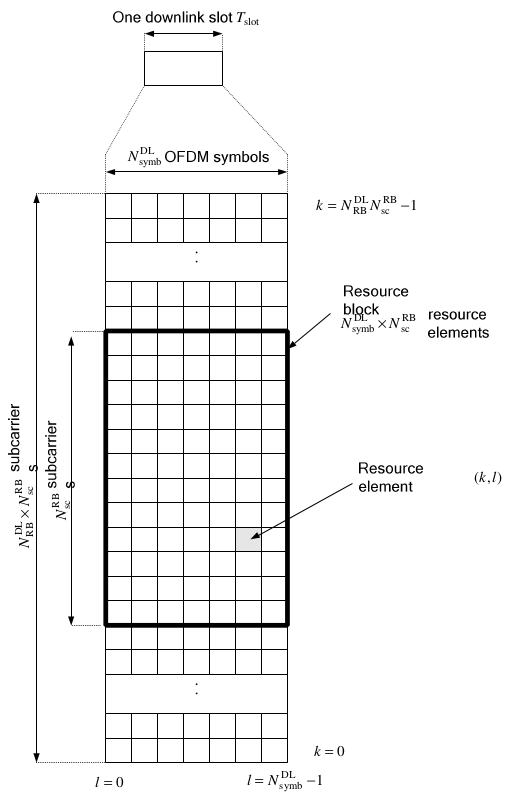
\includegraphics[height=4.5in]{res-grid}
	\caption{LTE downlink resource grid\cite{36series-211}}
\end{figure}

\begin{figure}[htbp]
	\centering
	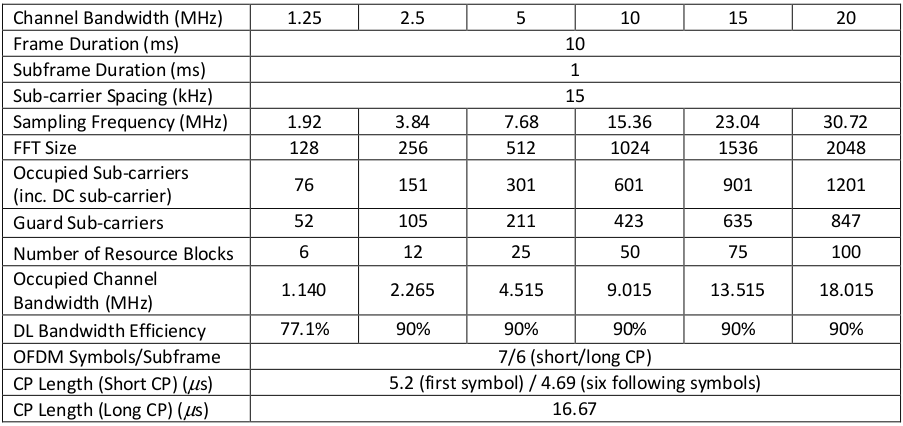
\includegraphics[height=2.5in]{ofdm-params}
	\caption{LTE downlink physical layer parameters\cite{nutshell}}
\end{figure}

\begin{figure}[htbp]
	\centering
	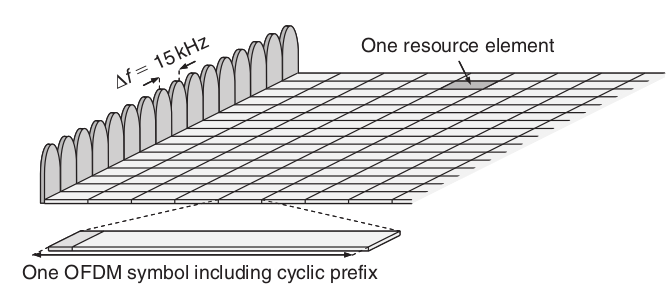
\includegraphics[height=1.5in]{DL-PHY-RES}
	\caption{LTE downlink physical resource}
\end{figure}

\begin{figure}[htbp]
	\centering
	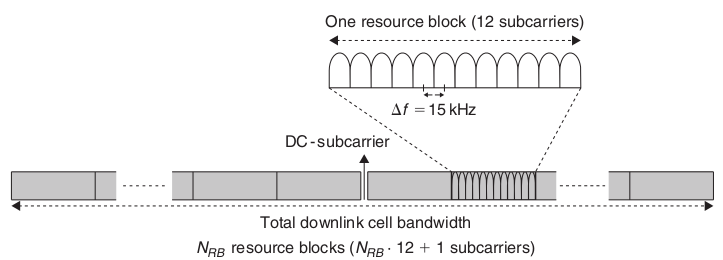
\includegraphics[height=1.5in]{DL-Frequency}
	\caption{Frequency-domain structure for LTE downlink}
\end{figure}

\begin{figure}[htbp]
	\centering
	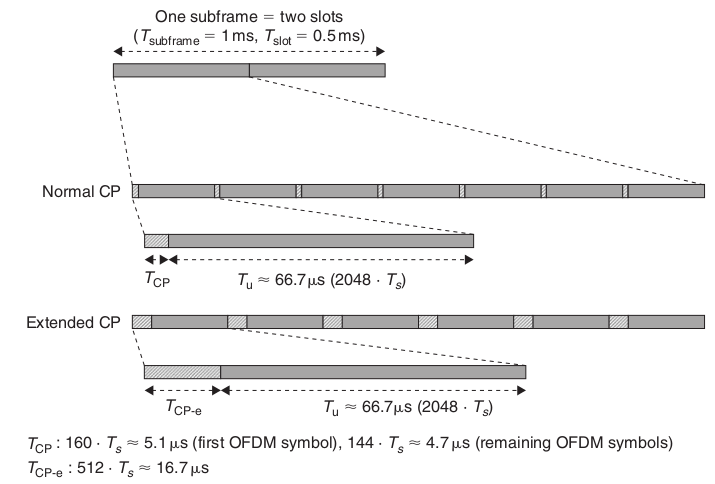
\includegraphics[height=3in]{DL-Time}
	\caption{Detailed time-domain structure for LTE downlink transmission}
\end{figure}

\begin{comment}
\section{LTE Downlink Simulator}
\end{comment}

\section{Benchmark Suite Implementation}

WiBench中解调的最大似然软输出映射成bit流的规则是:

\begin{verbatim}
"+"->"1"
"-"->"0"
\end{verbatim}

itpp库中的Turbo解码模块认为其输入输出是“+1”或“-1”,因此如果输入是bit流,首先要做如下映射:

\begin{verbatim}
"1"->"-1"
"0"->"1"
\end{verbatim}

而如果输入是软值,则认为正值代表“+1”,负值代表“-1”。因此,在目前的实现中,解调与解码的软值与bit的映射规则恰好相反,所以将解调模块的输出作为解码模块的输入之前,首先要做一个符号取反操作。

\bibliographystyle{plain}
\bibliography{../ref}

\end{document}


